\documentclass[12pt, twoside]{article}
\usepackage{jmlda}
\newcommand{\hdir}{.}
\usepackage[utf8]{inputenc}
\usepackage[english,russian]{babel}
\usepackage{graphicx}
\usepackage{minted}
\usepackage[linesnumbered,boxed]{algorithm2e}
% \usepackage{algorithm}
% \usepackage{algpseudocode}
% \usepackage[usenames]{color}
% \usepackage{colortbl}





\begin{document}

\title
    [Шаблон статьи для публикации] % краткое название; не нужно, если полное название влезает в~колонтитул
    {Распознавание текста на основе скелетного представления толстых линий и сверточных сетей}
\author
    { И.\,А.~Рейер, В.\,В.~Стрижов, М.\,C.~Потанин, Д.~Ожерелков, А.~Булатов, В.\,А.~Шокоров}

\email
    {reyer@forecsys.ru; strijov@gmail.com; mark.potanin@phystech.edu; ozherelkov97@gmail.com; ayd98@mail.ru; v.shokorov@yandex.ru}
% \thanks
%     {}
% \organization
%     {$^1$Организация, адрес; $^2$Организация, адрес}
\abstract
    {
    	Исследуется метод распознавания символа, по его скелетному представлению, с приминением сверточных нейронных сетей на графе скелета. В качестве входных данных используется скелетное представление символа, например, его можно получить используя Алгоритм Л.М.Местецкого. Предложеный алгоритм позволяет работать с графами небольшого размера, количество вершин которого не больше 30. Наша модель показала результат качества сравнимый с результатом человека. Также предложенный алгоритм имеет достаточно легкую с вычислительной точки зрения структуру и позволяет обрабатывать один граф за $0,3 \mu s$.
    %   В ряде экспериментов...
        % \textcolor{gray}{Так же рассматривается задача привилегированного обучения, когда происходит совместная минимизация ошибки двух сетей, более сложной, но классической CNN и более легкой GCNN. Целью исследования является анализ изменения весов GCNN.}
        Проведены эксперименты по классификации рукописных цифр.
    	
\bigskip
\noindent
\textbf{Ключевые слова}: \emph {распознавание текста, скелетное предствавление, GCNN, привилегированное обучение}
}


%данные поля заполняются редакцией журнала
% \doi{10.21469/22233792}
% \receivedRus{01.01.2017}
% \receivedEng{January 01, 2017}

\maketitle


\section{Введение}

Мы решаем задачу распознавания текста, для этого рассматриваем изображения символа, как двумерную фигуру, ограниченной конечным множеством полигонов. Алгоритм Л.М.Местецкого, основанный на прямом построении обобщенной триангуляции Делоне Множества граничных элементов фигуры позволяет нам получить скелетное графовое представление данного символа, с достаточным качеством точности положения вершин.
Цель исследования изучить возможность применения сверточной нейронной сети на скелетном представлении символа. Мы рассматриваем изображения символа, как двумерную фигуру, ограниченной конечным множеством полигонов, полученной из бинаризации изображения (В нашем случае под бинаризацией понимается следующее: все пиксели, цвет которых НЕ черный (в нотации цветов от 0 до 255), становятся белыми). Алгоритм Л.М.Местецкого~\cite{Mestetskiy_alg} позволяет нам получить скелетное графовое представление данного символа, поэтому исследовательская часть нашей работы заключается в том, чтобы научиться качественно преобразовывать графовое представление символа в вектор, для дальнейшего решения задачи классификации.
Сложность данного подхода заключается в нерегулярности структуры графа, объекты, подлежащие обработке, не упорядочены и могут иметь произвольную размерность и структуру связей. Обстоятельное исследование этой проблемы и возможных подходов к ее решению можно найти в статье~\cite{going_beyond_Euclidean_data}. Кроме канонического решения задачи обработки изображения CNN, похожая проблема решается в~\cite{solution_by_SVM_classifier} там используется набор контуров и граф скелетного представления с последующим линейным классификатором SVM. Также существует подход использующий медиальное представление~\cite{solution_by_Medial_Representation_GCNN}. Существует ряд статей Липкиной А.Л. и Л.М.Местецкий Посвященных решению нашей задачи, например~\cite{Lipkina_Mestetskiy_1},~\cite{Lipkina_Mestetskiy_2}.


% Решаемая в данной работе задача
Для решения задачи необходимо найти оптимальные параметры графового представления (такие как координаты вершин, их валентность, степень, тольщина линий и тд.) описывающие символ, для их подбора можно воспользоваться например \cite{Structural_functional_analisys}.
% Предлагаемое решение
% Работа или работы описывающие наиболее близкие решения
% Анализ сильных и слабых сторон предлагаемого решения
% Цель эксперимента, на каких данных будет выполнен эксперимент
\section{Свертка на графе}
Многие подходы созданные для свертки на графе предназначены либо для предсказания существования ребра между вершинами, известное, как Link Prediction, либо для классификации вершин (Node Classification). На самом деле это схожие задачи, потому что они решаются через представление вершину в виде вектора, для дальнешего сравнения расстояния между ними. Эти методы описания основываются на структуре связей и требуют, чтобы каждая вершина либо имела только одну метку, либо не имела вовсе, отсюда следует, что локальное описание графа должно быть разнообразно, что не выполняется в нашем случае, т.к. скелетонизация выдает граф, вершины которого часто имеют степень равную двум, и количество вершин в графе редко превышает 25, и вдобавок каждая вершина имеет 4 метки. Таким образом получаем, что известные методы плохо применимы для решения данной задачи.

Интересный подход был описан в статье~\cite{embend_like_cnn_on_photo}, там предлагался алгоритм сжатия графа состоящий из трех частей: сначала применяется node2vec~\cite{node2vec}, затем на полученном векторном представлении вешин используется PCA (principal component analysis), что позволяет получить значимые "направления" верши графа, иными словами показать общий вид вершин графа, после чего, можно кслассифицировать полученное представление.

В статье про GraphSAGE~\cite{GraphSAGE}, был предложен метод, который решает задачу представления вершины в виде вектора, там используеются модификация рекурентной нейронной сети, следующее значение вектора вершины представляется как нелинейная функция от старого значения и агрегированных значений соседей. Такой подход позволяет использовать в качестве метки вектор неединичной длины, но, как заявляют авторы, метод работает не графах с более чем $100 000$ вершинах.

\begin{figure}[h]
\center{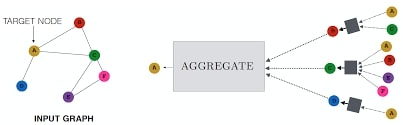
\includegraphics[width=0.6\textwidth]{pictures/GraphSage.jpg}}
\caption{Пример схемы свертки в статье про GraphSAGE.}
\label{GraphSage_scheme}
\end{figure}


% \begin{figure}[h]
% \center{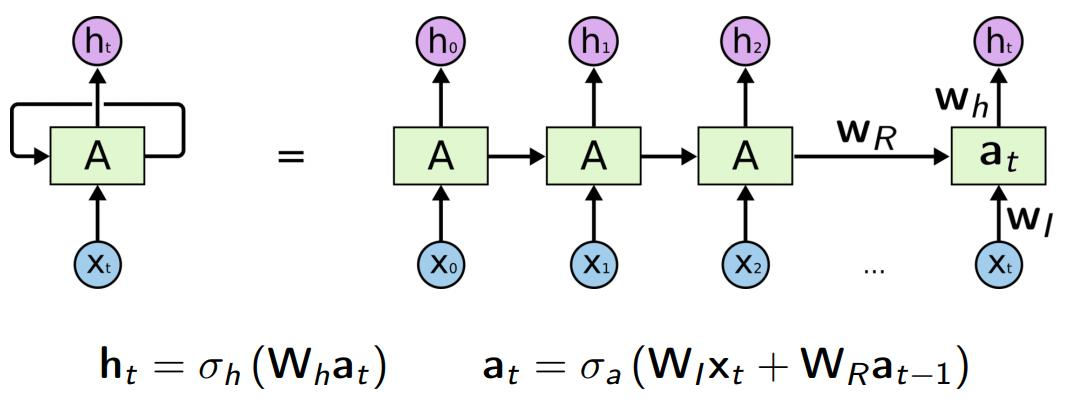
\includegraphics[width=0.9\textwidth]{pictures/rnn_scheme.jpg}}
% \caption{Общая схема рекуррентной нейронной сети.}
% \label{rnn_scheme}
% \end{figure}

\section{Постановка задачи}
% Ставим задачу формально для того, чтобы предложить оптимальный алгоритм ее решения.
Пусть дано множество $\mathcal{A}$, состоящее из пар~$(\mathbf{I}, y)$, где $\mathbf{I} \in \mathbb{I} $ - растровая черно-белая картинка размера~$m\times n$ пикселей, в нотации цветов от 0 до 255, с изображением рукописной цифры, а $y \in \mathbb{Y}$ - метка класса - значение цифры. Примером набора таких даных, например, является-MNIST~\cite{mnist_explanation}. 

Задача заключается в построении модели, которая определяет по изображению цифры ее значание. Предлагаеммый подход заключается в использовании скелетонизации, для получения графового описания изображения, графовой сверточной сети, для представления графа в виде вектора фиксированной длины, полносвязной нейронной сети, для классификации полученного представления графа. 

Для описания решения задачи зададим пространство неориентированных графов~$G$, полученных с помощью скелетного представления $f_1\colon \mathbf{I} \to \mathbf{G} \in G$, причем каждой вершине графа соответствует $\mathbf{l} \in \mathbf{L} = \mathbb{R}^4_+$, 4 числа, называемыми координатами вешины, радиусом и количеством соседей. Координатами вершины является два числа, описывающие положение вершины на изобрадении, радиусом называется максимальный размер окружности, которую можно вписать в фигуру, представленной на бинаризованном изображении цифры.

При данной формулировке, задача разбивается на несколько подзадач, первая, нахождение оптимального представление изображения в виде графа, вторая, нахождение оптимальной модели для предсказания класса графа, другими словами какому классу принадлежит обрабатываемое изображение.
\subsection{Описание подзадачи о представлении изображения графом}
Для данной части используется алгоритм Л.М. Местецкого.
%  FIXME описать нормально задачу из алгоритма Местецкого
\subsection{Описание подзадачи о классификации графа}
Для этой части рассматривается множество сверточных графовых нейронных сетей $\mathfrak{C} = \{ \mathbf{C}_1, \mathbf{C}_2, \dots\}$ и положительное целое число $\delta$ (т. е. ожидаемое количество классов $= |\mathbb{Y}|$), мы хотим получить  $\overrightarrow{\mathbf{d}} - \delta$-мерное представление для каждого графа $\mathbf{G}_i \in \mathfrak{C}$, где $\forall i, \overrightarrow{\mathbf{d}_i}$ соответствует вероятности принадлежности этого графа к $i$-му классу из $\mathbb{Y}$.

Рассматриваются графы, $\mathbf{G} = (\mathbf{N}, \mathbf{E}, \lambda)$, где $\mathbf{N}$-множество вершин, а $\mathbf{E} \subseteq (\mathbf{N}\times \mathbf{N})$-множество ребер. Также для графа $\mathbf{G}$, должна существовать функция $\lambda$ такая, что $\lambda\colon \mathbf{N} \to \mathbf{l}$, которая присваивает уникальную метку из множества $\mathbf{L}$ каждому узлу $\mathbf{n} \in \mathbf{N}$.

При данных условиях, постановка задачи выражается через минимизацию перекрестную энтропию между прогнозируемым и фактическим значение, т.к. Cross-Entropy Loss используется для создания уверенной модели, т.е. модели не только точно предсказывающей значение метки класса, но и делающей это с большей вероятностью.
\begin{equation}
\label{g2v_overview_loss}
    \argmin_{\mathbf{C} \in \mathfrak{C}} -\sum \sum_i^\delta \mathbf{d}_i\log \mathbf{y}_i
\end{equation}
Где первая сумма берется по всем парам $(\mathbf{I}, y)$ из множества $\mathcal{A}, \mathbf{I} \in \mathbb{I}, y \in \mathbb{Y}, \mathbf{d} = \mathbf{C}(\mathbf{I})$ - $\delta$-мерное представление для графа, $\mathbf{y}$ - вектор, $y$-ая координата которого $= 1$, остальные~$=0$.

Таким образом задача заключается в минимизации~(\ref{g2v_overview_loss}) для графовой сверточной сети, общий вид которой показан на рис.~\ref{my_g2v_scheme}, схема каждой состовляющей показана на рис.~\ref{rnn_scheme},~\ref{fcnn_scheme} соответственно. 

\section{Описание базового алгоритма}
В качестве базового алгоритма взят подход из статьи~\cite{base_alg}, идея которого заключается в том, что вершинами искомого графа являются пиксели, поэтому каждая вершина получается с небольшим количеством соседей и данный граф имеющими схожую структуру, что и изображение, и в качестве свертки на вершинах используется линейное преобразование от векторных описаний соседей. Отличие данного алгоритма от сверточной нейронной сети заключается в том, что сеть оперирует понятиями присущими графу, другими словами на вход подается матрица смежности и метка на каждой вершине. Такой подход позволяет достичь точности на базе данных MNIST~\cite{mnist_explanation} $92\%$


Базовый алгоритм также решает на задачу минимизации~(\ref{g2v_overview_loss}), также находит минимум на множестве $\mathcal{A}$, состоящее из пар $(\mathbf{I}, y)$, при этом операция свертка происходит на вершинах, которые являются пикселями самого изображении. Получаем, что задача переписывается в виде:
\begin{equation}
\label{cnn_overview_loss}
    \argmin_{\mathbf{w}} -\sum \sum_i^\delta \mathbf{d}_i\log \mathbf{y}_i
\end{equation}
Где минимизация идет по всем весам сверточной сети, первая сумма берется по всем парам $(\mathbf{I}, y)$ из множества $\mathcal{A}$.


\section{Описание алгоритма}
Нами был предложен алгоритм решения задачи классификации графа скелетного представления, состоящий из 3 частей. Первая, свертка на графе, сделанная на подобии GraphSAGE, данную часть алгоритма можно увидеть на схеме~Алгоритм~\ref{GCNN_alg}, вторая выделение главных компонент, по аналогии с graph embend like cnn on photo, затем, полносвязныйе слои для классификации полученных компонент. Общую схему алгоритма c применением PCA можно увидеть на рис.~\ref{my_g2v_scheme}. Так как PCA достаточно дорогостоящая по времени опперация, поэтому, после того, как сеть достаточно обучилась, мы находим все главные компоненты, для каждого класса графа, усредняем их и заменяем PCA на разложение вектора, описывающего какую-то вершину, на координаты в базисе усредненных главных компонент. Модифицорованную общую схему алгоритма можно увидеть на рис~\ref{my_g2v_next_csheme}.
\begin{figure}[h]
\center{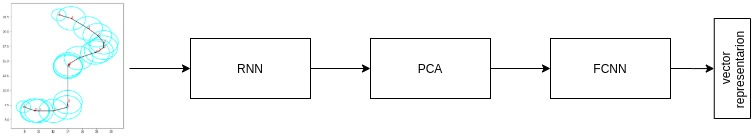
\includegraphics[width=0.8\textwidth]{pictures/my_g2v_scheme.jpg}}
\caption{Общая схема нейронной сети c применением PCA.}
\label{my_g2v_scheme}
\end{figure}

\begin{figure}[h]
\center{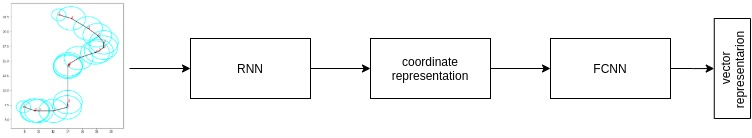
\includegraphics[width=0.8\textwidth]{pictures/my_g2v_next_csheme.jpg}}
\caption{Общая схема нейронной сети без использования применением PCA, в данном случае PCA заменяется на координатное представление каждого вектора описывающего вершину.}
\label{my_g2v_next_csheme}
\end{figure}
\begin{algorithm}[H]
\SetAlgoLined %% Это соединяет линиями логические части
\Input{\textbf{input : }Граф $\mathbf{G} = (\mathbf{N}, \mathbf{E}, \lambda)$, напомним, что функция $\lambda\colon \mathbf{N} \to \mathbf{l}$ задает метки на вершинах; глубина расспространения $K$; матрица весов $\mathbf{W}^k, \forall k \in \{1\dots K\};$ нелинейная функция $\sigma$; дифференцируемая агрегирующая функция $\mathrm{AGGREGATE}_k, \forall k \in \{1\dots K\}$; функция описывающая соседей $\mathcal{N} \colon n \to 2^n, \mathcal{N}(n) = \{m \in \mathbf{E} \colon (m, n) \in \mathbf{E}\}$}

\Output{\textbf{output : }векторное представление $\mathbf{z}_n \ \forall n \in \mathbf{N}$}

$h^0_n \leftarrow \lambda(n), \ \forall n \in  \mathbf{N}$;

\For{ $k = 1\dots K $}{
    \For{ $n \in \mathbf{N} $}{
        $h^k_{\mathcal{N}(n)} \leftarrow \mathrm{AGGREGATE}_k (\{ h^{k-1}_m, \ \forall m \in \mathcal{N}(n) \});$ \\ 
        $h^k_n \leftarrow \sigma \big ( \mathbf{W}^k \cdot \mathrm{CONCAT} ( h^{k-1}_n, h^{k-1}_{\mathcal{N}(n)} \big );$
    }
    $h^k_n \leftarrow h^k_n / \|h^k_n\|_2, \ \forall n \in \mathbf{N}$
} 
$\mathbf{z}_n \leftarrow h^K_n, \ \forall n \in \mathbf{N}$
\caption{Псевдокод для сверточной сети на графе}
\label{GCNN_alg}
\end{algorithm}

\section{Вычислительный эксперимент}
\subsection{Данные}
В качестве первичного набора данных используется библиотека MNIST~\cite{mnist_explanation}. Перед скелетизацией изображения были бинаризованы(все символы, не являющиеся совершенно черными, переводятся в белые), поскольку этого требует алгоритм скелетизации. Полученный скелет, являющийся ненаправленным графом, каждая вершина описывается координатами, степенями вершин и максимальными радиусами кругов, вписанных в цифры.
\subsection{Приминение предложенного алгоритма}
После скелетонизации, на полученных графах обучается предложенная сеть, первая проблема, с которой мы сталкиваемся при обучении это то, что необходимо правильно инициализировать веса свертки, так как если у нас веса инициализированны случайно, то получится, что алгоритм который используется для PCA не будет сходиться, потому что рассматриваемые графы имеют достаточно однородную структуру, поэтому вектора вершин все будут сонаправленны. Это решается несколькими запусками обучения. Далее, когда кривая ошибки сходится, (на данном этапе у нас точность предсказания равна $55\%$), после этого мы заменяем PCA на координатное представление и дообучаем сеть. 

В ходе эксперимента подбираются оптимальные параметры сети такие как, число нейронов в скрытом слое, глубина работы алгоритма свертке на графе, функции активации и т.д. После чего мы получаем итоговую точность предсказания порядка $77\%$.

\section{Анализ ошибки}
На рисунке~\ref{heat_maps}(а) показанна гистограмма определения класса нашего алгоритма, по оси $y$ отображаются истинные значения класса, по оси $х$ предсказанный алгоритмом класс. На рисунке~\ref{heat_maps}(б) показанна подобная гистограмма, кроме главной диагонали, отсюда видно, что алгоритм часто путает, например, 8 и 9. 
\begin{figure}[h]
\begin{minipage}[h]{0.49\linewidth}
\center{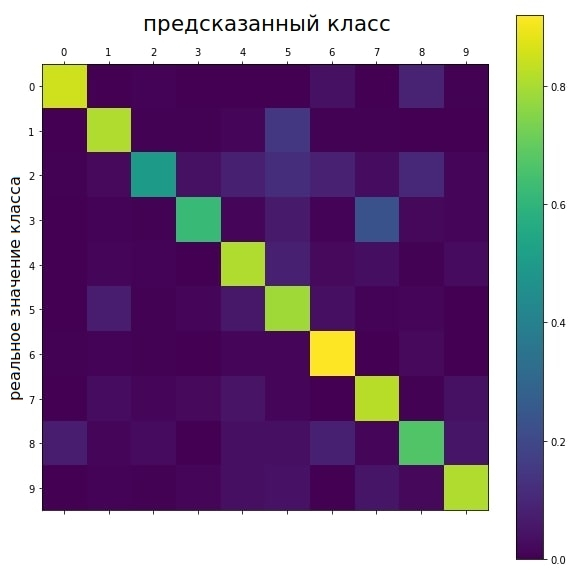
\includegraphics[width=0.8\textwidth]{pictures/heat_map_new.jpg} \\ а)}
\end{minipage}
\hfill
\begin{minipage}[h]{0.49\linewidth}
\center{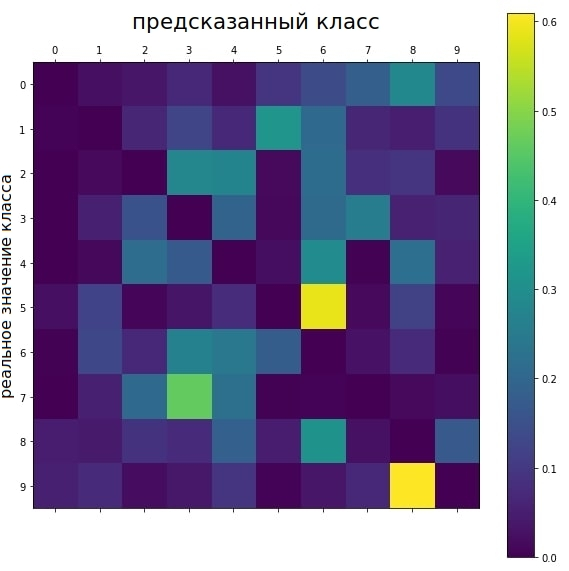
\includegraphics[width=0.8\textwidth]{pictures/heat_map_new_background.jpg} \\ б)}
\end{minipage}
\caption{гистограмма определения класса нашего алгоритма, по оси $y$ отображаются истинные значения класса, по оси $х$ предсказанный алгоритмом класс. На рисунке~(б) показанна подобная гистограмма, кроме главной диагонали, отсюда видно, что алгоритм часто путает, например, 8 и 9.}
\label{heat_maps}
\end{figure}

Достаточно показательным фактом оказалаось то, что ответ сети оказался инвариантным относительно сдвига координат вершин, что соответствует логике. Так же если просмотреть особые случаи, то на мнигих входных данных даже человеку сложно определить истинное значение цифры, примеры таких вхдных данных можно рассмотреть на рис.~\ref{incorrect_input}. Приведя небольшое исследование мы определили, что человек по скелетному представлению может верно определить класс с точностью $84\%$, полученную гистаграмму можно увидеть на рис.~\ref{my_results}.

\begin{figure}[h]
\center{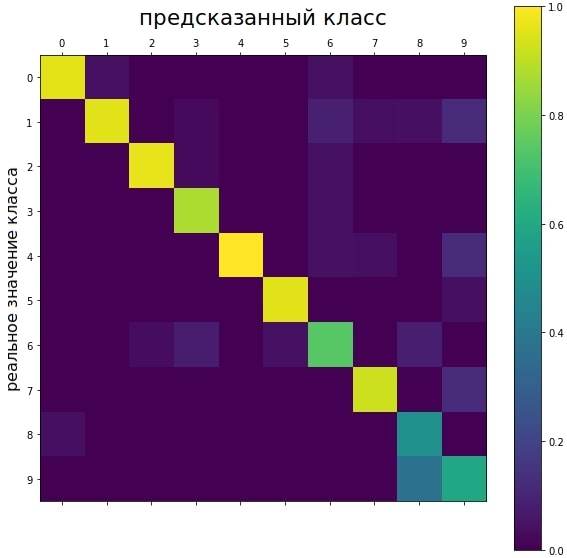
\includegraphics[width=0.392 \textwidth]{pictures/my_results.jpg}}
\caption{гистограмма определения класса человеком, по оси $y$ отображаются истинные значения класса, по оси $х$ предсказанный алгоритмом класс.}
\label{my_results}
\end{figure}

\begin{figure}[H]
\begin{minipage}[H]{0.47\linewidth}
\center{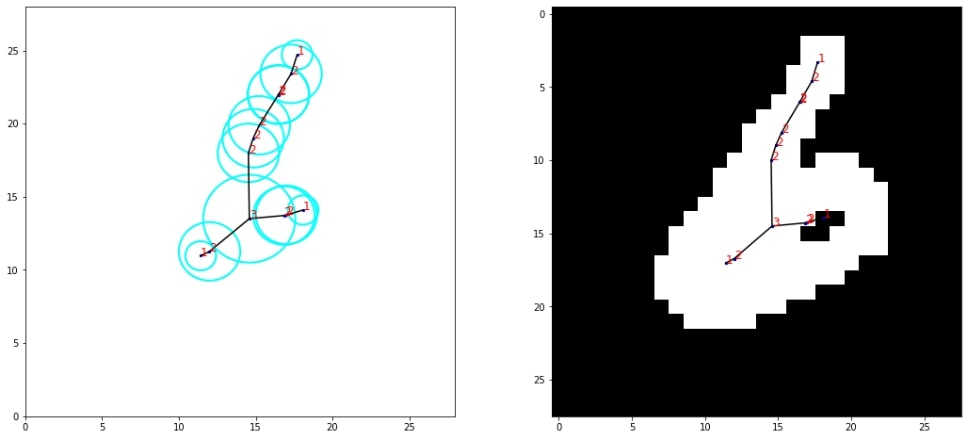
\includegraphics[width=1\linewidth]{pictures/6->1_example.jpg}} истинное значение класса - 6 \\
\end{minipage}
\vfill
\begin{minipage}[H]{0.47\linewidth}
\center{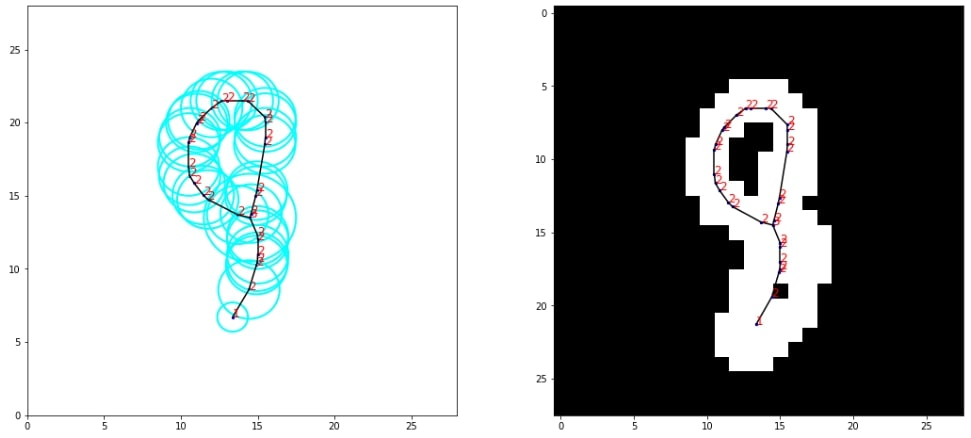
\includegraphics[width=1\linewidth]{pictures/8->9_example.jpg}} истинное значение класса - 8) \\
\end{minipage}
\vfill
\begin{minipage}[H]{0.47\linewidth}
\center{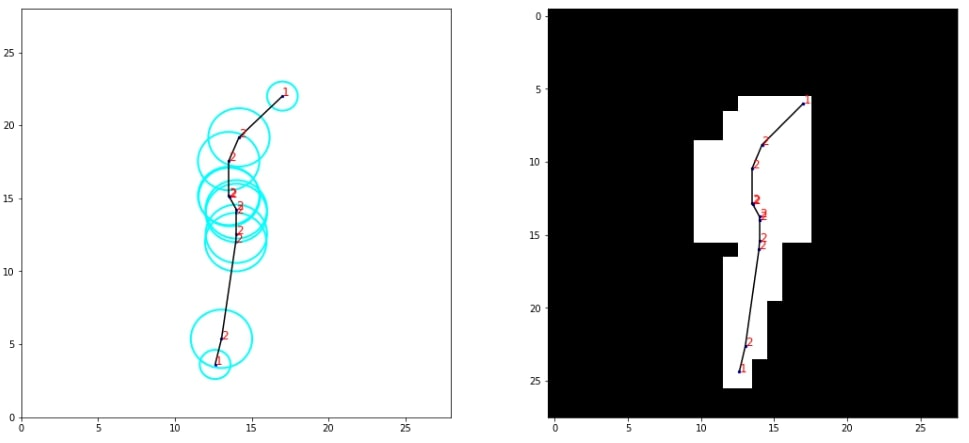
\includegraphics[width=1\linewidth]{pictures/9->?_example.jpg}} истинное значение класса - 9) \\
\end{minipage}
\caption{Примеры скелетных представлений, которые по которым невозможно верно определить истинный класс.}
\label{incorrect_input}
\end{figure}



\bibliographystyle{unsrt}
\bibliography{References}






\end{document}